\section{Cara Menggunakan Buku Ajar}

Pembelajaran disarankan dilakukan secara berurutan dari Bab I hingga Bab X (dan bab tambahan jika tersedia), karena setiap konsep dibangun di atas materi sebelumnya. Bab II menjadi fondasi teoretis, Bab III memperkuat matematika kriptografi, dan bab-bab berikutnya berfokus pada implementasi serta analisis keamanan yang lebih kompleks.

\subsection{Alur Pembelajaran yang Kohesif}

Setiap bab dirancang untuk menjadi landasan bagi bab berikutnya:
\begin{itemize}
  \item \textbf{Bab II} memberikan \textit{big picture} keamanan informasi yang menjawab "mengapa kita perlu kriptografi?"
  \item \textbf{Bab III} menjawab "bagaimana matematika membuat kriptografi mungkin?" dengan fondasi yang akan digunakan langsung di Bab IV
  \item \textbf{Bab IV} menerapkan matematika Bab III dalam cipher klasik, mempersiapkan Anda untuk algoritma modern di Bab V
  \item \textbf{Bab V-VII} membangun dari cipher klasik ke algoritma modern, dengan matematika yang semakin kompleks
  \item \textbf{Bab VIII-IX} mengintegrasikan semua konsep dalam protokol dan analisis keamanan nyata
\end{itemize}

\subsection{Struktur OBE untuk Pembelajaran Terukur}

Gunakan struktur OBE di setiap bab sebagai panduan belajar. Komponen utama yang perlu diikuti adalah:
\begin{itemize}
  \item \textbf{Sub-CPMK}: target kompetensi yang harus dicapai
  \item \textbf{Materi Pokok}: teori, contoh numerik, dan kode C
  \item \textbf{Aktivitas Pembelajaran}: praktikum, diskusi, atau studi kasus
  \item \textbf{Latihan}: penguatan konsep sebelum asesmen
  \item \textbf{Asesmen}: alat ukur pencapaian Sub-CPMK
  \item \textbf{Checklist}: evaluasi diri setelah belajar
\end{itemize}

\subsection{Koneksi Teori dan Praktik}

Setiap bab dirancang dengan keseimbangan antara:
\begin{itemize}
  \item \textbf{Teori}: Konsep matematis dan prinsip kriptografi
  \item \textbf{Implementasi}: Kode C yang menunjukkan bagaimana teori bekerja dalam praktik
  \item \textbf{Analisis}: Mengapa suatu desain aman atau tidak
\end{itemize}

Agar pembelajaran konsisten, alokasikan waktu belajar secara proporsional antara membaca materi, praktik, latihan, dan refleksi. Grafik berikut bersifat ilustratif dan dapat disesuaikan dengan kebutuhan belajar masing-masing mahasiswa.

\begin{figure}[htbp]
  \centering
  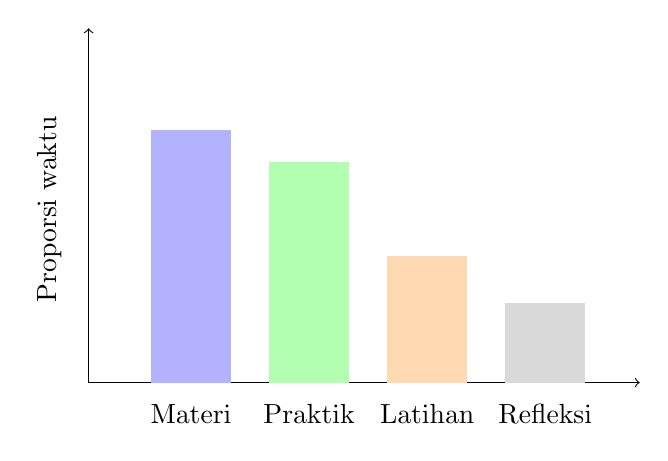
\begin{tikzpicture}
    \draw[->] (0,0) -- (0,4.5);
    \draw[->] (0,0) -- (7,0);
    \filldraw[blue!30] (0.8,0) rectangle (1.8,3.2);
    \filldraw[green!30] (2.3,0) rectangle (3.3,2.8);
    \filldraw[orange!30] (3.8,0) rectangle (4.8,1.6);
    \filldraw[gray!30] (5.3,0) rectangle (6.3,1.0);
    \node at (1.3,-0.4) {Materi};
    \node at (2.8,-0.4) {Praktik};
    \node at (4.3,-0.4) {Latihan};
    \node at (5.8,-0.4) {Refleksi};
    \node[rotate=90] at (-0.5,2.2) {Proporsi waktu};
  \end{tikzpicture}
  \caption{Ilustrasi proporsi waktu belajar per komponen (dapat disesuaikan).}
\end{figure}
